% reviewers: Zam, Jared?

\documentclass{article}
\usepackage{graphicx}

\begin{document}

\title{Streaming approaches to error detection and trimming in the analysis of
short sequencing reads}
\author{TBD}
\maketitle

\section{Introduction}

K-mer spectral analysis is a powerful approach to error detection and
correction in shotgun sequencing data that uses k-mer abundances to
determine likely errors (cite Pevzner, Quake, khmer-counting paper).
Approaches derived from spectral analysis can be very accurate: Zhang
et al. (2014) show that spectral analysis is considerably more
effective at finding errors than quality-based approaches (cite).  However,
spectral analysis is also very compute intensive; most implementations
must count k-mers across entire sequencing data sets, which can be
memory- or I/O-intensive for large data sets.

Streaming algorithms can offer improved algorithmic and computational
efficiency in the analysis of large data sets (cite).  Streaming
algorithms typically examine the data only once, and scale in memory
usage sublinearly with respect to the input data.  Streaming
algorithms have not been applied to k-mer spectral analysis of reads,
although XXX (melsted).

Brown et al. (2012) introduced a streaming algorithm for normalizing
k-mer abundance spectra, termed ``digital normalization'' (abbreviated
as ``diginorm'').  This procedure estimates the k-mer coverage of each
read in an online algorithm, by calculating the median k-mer abundance
of the read given all previous reads; reads above a certain estimated
coverage are set aside and their k-mers are not tracked.  This
algorithm is both online and {\em streaming} because it only collects
k-mers in reads with a low estimated coverage; for the same reason, it
is sublinear in memory for high coverage data sets.  The net effect of
diginorm is to reduce the data set size that must be considered for
downstream processing, such as {\em de novo} assembly (cite trinity,
elijah, etc.)

Here we develop a streaming algorithm for k-mer spectral analysis,
based on digital normalization, that can detect and remove errors in
sequencing reads.  This algorithm operates in sublinear memory, and
examines the data at most twice.  The approach offers a general
framework for making use of locus-specific graph saturation and could
potentially be used for error correction, variant calling, and a
streaming implementation of assembly.  Moreover, it can be applied to
data sets with variable coverage such as transcriptomes, metagenomes,
and amplified genomic DNA.

\section{Results}

\subsection{Coverage-normalized data can be used to locate
and correct errors in high-coverage shotgun sequencing data}

Our initial question was whether spectral error analysis could be
applied to genomic short read data after digital normalization.  We
tested this on a synthetic data set and an {\em E. coli} data set.  We
then compared the performance of Quake on the raw and digitally
normalized counts from the {\em E. coli data}.

\paragraph{Simulated data:}
We first applied digital normalization to a simulated data set with
known errors.  We generated the synthetic data set from a simulated
low-complexity genome (``simple genome''; see Methods for generation
and Table~\label{tab:data} for data set details). We then applied
digital normalization to these synthetic reads, normalizing to a
median 20-mer coverage of 20 (k=20, C=20).

The k-mer spectrum before and after digital normalization is shown in
Figure~\ref{fig:spectrum}.  While the total number of k-mers decreased
in the digitally normalized data set, the separation between the high
count k-mers and the low-count k-mers remains clear.  The key concept
underlying k-mer spectral error analysis is that in a high-coverage
data set, these high count k-mers will represent {\em correct} k-mers,
while the low count k-mers are produced by errors in the reads.
Simple classification methods suffice to identify and trim or correct
these low-count k-mers.

\begin{figure}[!ht]
 \centerline{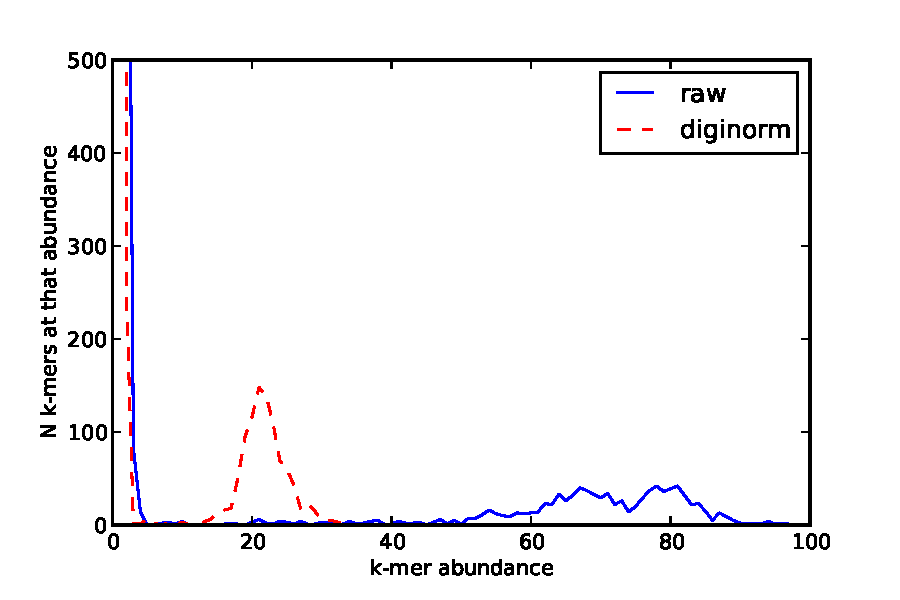
\includegraphics[width=4in]{./figures/kmer-spectrum}}
\caption{\bf K-mer spectrum of a simple artificial data set, before and after digital normalization.  The peaks at 1 represents erroneous k-mers resulting
from (simulated) error; the peaks centered at 80 (raw) and 20 (diginorm)
represent k-mers truly present in the genome which are present in many reads.}
\label{fig:spectrum}
\end{figure}

% note, need to put in diginorm #s. Or do we? In Methods, maybe?

%% make compare2

\begin{table}
\begin{tabular}{|l|c|c|l|}
\hline
Name & Origin & Number of reads & Description \\
\hline
simple genome & 10,000 & No repeats\\
{\em E. coli} MG1655 & 5,000,000 & Subset of NCXXXXX \\
simple metagenome & 2,347 & Dynamic range of YYY \\
simple transcriptome & 568 & Dynamic range of ZZZ; multiple exons\\
\hline
\end{tabular}
\label{tab:data}

\caption{Data sets used}
\end{table}

We next used k-mer counts from the downsampled read set to detect
errors in the original read set.  The algorithm is straightforward: we
look for bases at the beginning or ends of low-abundance runs of
k-mers in each read. We used a ``trusted k-mer'' cutoff of $C_0 = 3$
as our abundance cutoff, below which we assumed k-mers were erroneous
(see Methods).  The results are presented in Table~\ref{tab:a}.  Of
the 531 simulated reads from the simple genome containing one or more
errors, predicted errors matched the known truth exactly for 443 of
them (true positives), and 466 reads were correctly predicted to
contain no errors (true negatives). 0 reads were falsely predicted to
have no errors (false negatives). The errors in 88 reads were
miscalled -- while the reads each had one or more errors, the
positions were not correctly called -- and three reads were
incorrectly predicted to contain errors, leading to a total of 91
false positives.  Using the above definitions, we calculated the
prediction sensitivity to be 100\% and the prediction specificity to
be 83.0\%.

%% make compare6
%545 erroneous reads in simple-genome-errors-nodn.pos
%531 erroneous reads in simple-genome-reads.mut.pos
%440 reads in common => all error positions AGREE
%91 DISAGREE
%total # of reads: 1000
%TP: 440
%TN: 455
%FP: 105
%FN: 0
%sensitivity: 1.0
%specificity: 0.807339449541

When we applied spectral error detection to the unnormalized reads, we
saw similar results: 440 TP, 455 TN, 105 FP, and 0 FN, for a
sensitivity of 100\% and a specificity of 80.7\% (Table~\ref{tab:a}). The only difference
in parameters for this analysis was that we used a cutoff of $C_0=10$,
to account for the shifted k-mer spectrum from diginorm.

% @CTB here we could describe # of k-mers, etc.

\begin{table}
\begin{tabular}{|l|c|c|}
\hline
(Simple genome) & Raw counts & Diginorm counts \\
\hline
Perfect detection (TP) & 474 & 485 \\
No errors (TN) & 355 & 366 \\
Miscalled errors (FP) & 159 & 148 \\
Mispredicted errors (FP) & 12 & 1 \\
Missed errors (FN) & 0 & 0 \\
\hline
Sensitivity & 100\% & 100\% \\
Specificity & 73.5\% & 76.5\% \\
\hline
\end{tabular}
\label{tab:a}

\caption{Spectral error detection on 1000 synthetic reads from a
  simulated 10kb genome, using raw and digitally normalized
  counts.  The counts are the number of reads where all errors were
  detected perfectly (TP), no errors were present (TN), one or more errors were miscalled (one type of FP), errors were mistakenly called in an error-free read (the other type of FP), and errors present in a read were missed (FN). }
\end{table}

% make ecoli-report.txt

\paragraph{{\em E. coli} reads:}
We next applied digital normalization and k-mer spectral error
detection to an Illumina data set from {\em E. coli} MG1655 (cite
Chitsaz).  In real reads, we do not know the location of errors; to
calculate them, we mapped 5m untrimmed reads to the known {\em
  E. coli} MG1655 genome with bowtie1 (cite) and recorded mismatches
between the reads and the genome.  These mismatches were taken as
errors in the reads.  We found 8.0m errors in 2.2m reads, for an
overall error rate of 1.60\%.

We then compared the results of k-mer spectral error detection with
and without digital normalization.  We used the same parameters as on
the simulated genome.  The results are presented in
Table~\ref{tab:ecoli_dn_counts}. Using the raw counts, the
sensitivities were close -- using the raw counts, we achieved a
sensitivity of 72.0\%, versus 71.4\% using the counts from the
digitally normalized reads.  The specificities were also comparable --
43.5\% using the raw counts, and 42.9\% using the digitally normalized
counts.

\begin{table}
\begin{tabular}{|l|c|c|}
\hline
(E. coli) & Raw counts & Diginorm counts \\
\hline
Distinct k-mers & XXX & YYY \\
\hline
Perfect detection (TP) & 818,503 & 807,367 \\
No errors (TN) & 2,797,925 & 2,797,254 \\
Miscalled errors (FP) & 1,039,052 & 1,046,402 \\
Mispredicted errors (FP) & 25,499 & 26,170 \\
Missed errors (FN) & 319,021 & 322,807 \\
\hline
Sensitivity & 72.0\% & 71.4\% \\
Specificity & 43.5\% & 42.9\% \\
\hline
\end{tabular}
\label{tab:ecoli_dn_counts}

\caption{Spectral error detection on 5m {\em E. coli} reads, using raw and
  digitally normalized counts.}
\end{table}

% why such poor results on E. coli? repeats, or what?

\paragraph{{\em E. coli} error correction with Quake:}

While the results above suggest that simple spectral error detection
works equally well both before and after digital normalization, we
wanted to see if we could successfully perform a full error {\em
  correction} after digital normalization.  To evaluate this, we applied
the Quake error corrector to the data.  Because Quake permits the use
of a different k-mer counting table from the data being corrected,
we separately used the counts from the raw reads and the counts from
the digitally normalized reads to correct the raw reads (see Methods
for details).

The results of running Quake on the raw data using counts from the raw
or digitally normalized data are shown in Table~\ref{tab:quake_ecoli}.
The performance was essentially the same: Quake brought the overall
error rate in the data set from 1.60\% (8.0m errors) to
0.005\%-0.006\% (23,000 - 29,000 errors).

These results demonstrate that digitally normalized data retains all
of the information necessary for effective error correction with
Quake, despite having many fewer distinct k-mers.

%../pipeline/quake-ecoli-dn-cor.txt      ../pipeline/quake-ecoli-raw-cor.txt
% posfile ecoli-reads.dn.cor.sam.pos: 17119 mutated reads of 4906448; 22984 mutations total
% 450630551 bp total
% overall error rate: 0.005100%
%
% posfile ecoli-reads.raw.cor.sam.pos: 22380 mutated reads of 4907082; 29135 mutations total
% 450687634 bp total
% overall error rate: 0.006465%

\subsection{Coverage-normalized data can be used to locate errors in variable
coverage shotgun sequencing data}

One of the drawbacks of spectral abundance analysis is that it cannot
be directly applied to data with uneven coverage.  For example,
metagenomic or transcriptomic data sets typically contain reads from
both high-abundance and low-abundance molecules.  This variability in
coverage confounds naive spectral analysis for two reasons: first,
erroneous k-mers from very high abundance regions can accumulate and
increase in abundance over the threshold for trusted k-mers, thus
appearing to be correct; and second, correct reads from low coverage
regions yield k-mers below the trusted k-mer threshold and appear to
be incorrect.  In practice, therefore, error analysis for
metagenomic and transcriptome data uses other approaches.

Using digital normalization, we should be able to address both of these
problems.  First, by applying digital normalization to variable
coverage data and then working only with the k-mer counts from the
normalized reads, we can avoid counting high abundance errors.
And second, by ignoring reads with a low estimated coverage, we can
avoid misclassifying true low-abundance k-mers (Figure XXX).

% @algorithm?

% @graph with read abundance spectrum, showing which reads we will
% call errors in.

\paragraph{Simulated data:}
To test this approach, we generated two more synthetic data sets,
``simple metagenome'' and ``simple mRNAseq,'' which contain both high-
and low-abundance species (see Table~\ref{tab:data} for data set
details).  After generating synthetic reads with a 1\% error rate and
applying digital normalization (k=20/C=20), we again did spectral
error detection using the normalized counts.  However, this time we
modified the algorithm so that only reads with a median k-mer
abundance of 20 or greater were examined (see Methods).

% make mcompare2
% make rcompare2

\begin{table}
\begin{tabular}{|l|c||c|}
\hline
& simple metagenome & simple mRNAseq \\
\hline
Low coverage reads & 93 & 44 \\
\hline
Perfect detection (TP) & 978 & 228 \\
No errors (TN) & 1098 & 235 \\
Miscalled errors (FP) & 176 & 52 \\
Mispredicted errors (FP) & 6 & 9 \\
Missed errors (FN) & 2 & 0 \\
\hline
Sensitivity & 99.9\% & 100\% \\
Specificity & 84.7\% & 78.9\% \\
\hline
\end{tabular}
\label{tab:spectra_variable}
\end{table}

The results of running error detection on the synthetic metagenome and
mRNAseq data sets are shown in Table~\ref{spectra_variable}. For the
simple metagenome data set, 2254 of 2347 reads (96.0\%) met the
coverage criterion.  Of the 2254 reads analyzed, the errors in 978
erroneous reads were called perfectly (TP) and 1098 of the reads with
no errors were correctly called as error-free (TN).  2 reads were
incorrectly determined to be error free (FN).  Of the remaining 176
reads, 170 were miscalled (errors existed but were not exactly called)
and 6 were incorrectly called as erroneous when they were in fact
correct.  We calculated the prediction sensitivity to be 99.9\% and
the prediction specificity to be 84.7\%.  For the simple mRNAseq data
set, 524 of 568 reads (92.3\%) met the coverage criterion, with 228
true positives, 235 true negatives, 0 false negatives, and 61 false
positives, for a prediction sensitivity of 100.0\% and prediction
specificity of 78.9\%.  In both cases low-coverage reads were not
included in the statistics.

The results of the variable coverage error detection approach on
synthetic metagenomes and mRNAseq are comparable to the results
on the synthetic genome (100.0\% sensitivity and 83.0\%
specificity with the same parameters; Table~\ref{tab:a}).

% make rseq_compare2

\begin{table}
\begin{tabular}{|l|c||c|}
\hline
& Mock metagenome & mouse mRNAseq \\
\hline
Low coverage reads & 93 & 658,814 \\
\hline
Perfect detection (TP) & 978 & 71,315 \\
No errors (TN) & 1098 & 203,741 \\
Miscalled errors (FP) & 176 & 23,391 \\
Mispredicted errors (FP) & 6 & 24,464 \\
Missed errors (FN) & 2 & 18,275 \\
\hline
Sensitivity & 99.9\% & 79.6\% \\
Specificity & 84.7\% & 59.8\% \\
\hline
\end{tabular}
\label{tab:spectra_variable_real}
\end{table}

\paragraph{Mock metagenome data:}

\paragraph{mRNAseq data:}

We next applied variable coverage spectral error analysis to 1m mouse
mRNAseq reads (cite Trinity), with the same parameters as above.  Here
errors were again calculated by mapping the reads to the known
reference and finding mismatches. The results are shown in
Table~\ref{tab:spectra_variable_real}, third column.  We achieve
79.6\% sensitivity and 59.8\% specificity on the 340,000 high coverage
reads in this data set.

\paragraph{Error correcting variable coverage data with Quake:}

There are many sophisticated error correction algorithms implemented
for shotgun genome data, but relatively few work directly on
variable coverage data such as mRNAseq.  However, it should be possible
to apply genomic error correction to the high coverage components
of data sets after digital normalization.

To evaluate this, we applied Quake to the high coverage mRNAseq
reads.  We first extracted the 340,140 reads with estimated
high coverage (median k-mer coverage greater than or equal to 20)
from the mouse mRNAseq data set, and then digitally normalized the
data.  We next applied the Quake error corrector to the unnormalized
reads using the k-mer counts from the normalized reads, as with the
{\em E. coli} data set.

ZZZ.

\subsection{A streaming algorithm for error analysis}

Even with digital normalization, the spectral error detection approach
outlined above is a 2-pass offline algorithm for any given data set -
the first pass normalizes the read set and records the k-mer
abundances, while the second pass examines the reads.  A streaming
approach could avoid some or all of a second pass, leading to
greater efficiency.

Here we can make use of the redundancy of shotgun sequencing to avoid
examining much of the data twice. Shotgun
sequencing oversamples most regions -- for example, for a 100x
coverage genomic data set, we would expect 50\% or more of the genome
to be represented in more than 100 reads.  This is a consequence of
the Poisson-random sampling that underlies shotgun sequencing
(cite... Waterman?)  This oversampling provides an opportunity,
however; if we regard the read data set as a stream of incoming data,
some portions of the reference will more highly sampled earlier in the
stream than others.  For example, in mRNAseq, highly expressed
transcripts will on average be highly sampled much earlier than
low-expressed transcripts.

If highly sampled regions could be detected during iteration over the
read data set, we could apply the same approaches used above to do
error detection in a streaming fashion.  Digital normalization
provides such a method: by measuring coverage for each read against an
online De Bruijn graph, reads that reach a specified coverage
threshold can be examined for errors immediately.  Those reads that
had not yet reached high coverage could be set aside and re-examined
later.  This could result in significant runtime savings: for a
genomic data set with 100x coverage, no more than 20\% of the reads
would need to be examined twice.

The conceptual idea is presented in Figure~\ref{fig:concept}.  On the
first pass, low-coverage reads would be incorporated into the k-mer
database and set aside for later analysis, while high-coverage reads
would be analyzed for errors. On the second pass, the set aside reads
would be checked for coverage and either ignored or analyzed for
errors.  Crucially, this second pass will involve {\em at most}
another full pass across the data, but only if no reads were high
coverage in the first pass; the larger the high coverage component
of the data, the smaller the fraction of the data that is examined twice.

\begin{figure}[!ht]
 \centerline{\includegraphics[width=4in]{./figures/graph-saturation}}
\caption{\bf Diagram of streaming error detection. In a first pass
over the read data, reads are loaded in until the graph locus to which
they belong is saturated.  From that point on, reads are examined for
errors and not loaded into the graph.  In a second pass, only the subset
of reads loaded into the graph are examined for errors.}
\label{fig:concept}
\end{figure}

In Figure~\ref{fig:saturation}, we show diginorm-generated coverage
saturation curves for both real and error-free simulated reads from
{\em E. coli} MG1655.  In both cases, we see that by about 1m reads,
the majority of reads comes from loci with an estimated sequencing
depth of 20 or higher, and hence can be used for error analysis on the
first pass through the data.  Only those reads collected on the first
pass need to be examined again.

\begin{figure}[!ht]
 \centerline{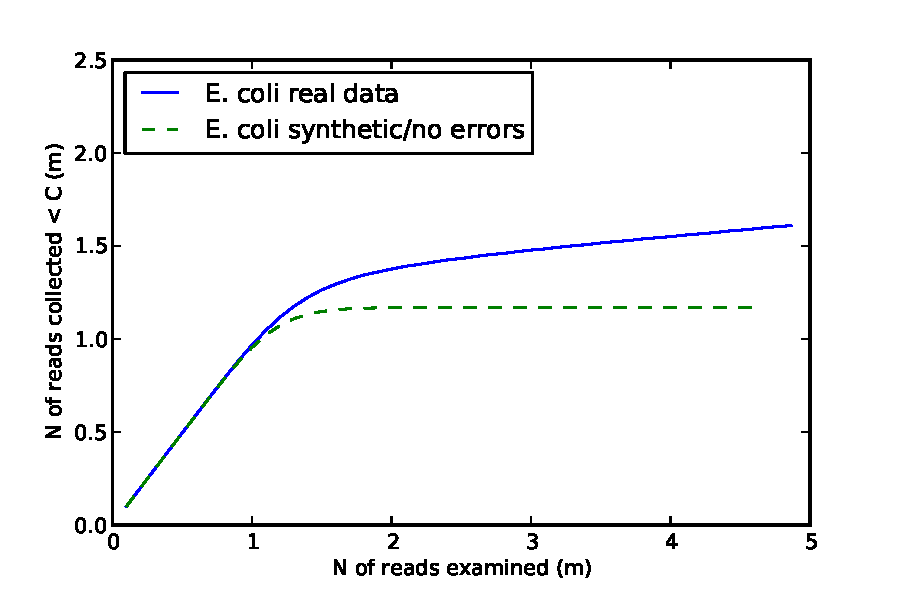
\includegraphics[width=4in]{./figures/saturation}}
\caption{\bf Saturation curve of a real and a simulated {\em E. coli} read data
set.  Reads are collected when they have an estimated coverage of less
than 20; in the early phase ($<$ 1m reads), almost all reads are
collected, but soon the majority of reads come from loci with an estimated
sequencing depth of $>$ 20 and are rejected.}
\label{fig:saturation}
\end{figure}

% make compare4
% make mcompare4
% make rcompare4

\begin{table}
\begin{tabular}{|l|c||c||c|}
\hline
& simple genome & simple metagenome & simple mRNAseq \\
\hline
Number of passes & 1.32 & 1.16 & 1.33 \\
\hline
Perfect detection (TP) & 485 & 977 (-1) & 228 \\
No errors (TN) & 365 (-1) & 1095 (-3) & 235 \\
Miscalled errors (FP) & 148 & 171 (+1) & 52 \\
Mispredicted errors (FP) & 2 (+1) & 9 (+3) & 9 \\
Missed errors (FN) & 0 & 2 & 0 \\
\hline
Sensitivity & 100.0\% & 99.9\% & 100.0\% \\
Specificity & 76.4\% & 84.4\% & 78.9\% \\
\hline
\end{tabular}
\label{tab:spectra_streaming}
\end{table}

When we apply this streaming approach to the simulated reads from the
``simple genome'', we obtain nearly identical numbers to the full two-pass
approach: 485 TP, 365 TN, 150 FP, and 0 FN, for a sensitivity of 100\%
and a specificity of 76.3\%.  However, only 320 of the 1000 reads are
examined twice - hence, it is a 1.32x pass algorithm on this data set.
Likewise, for the ``simple metagenome''
and ``simple mRNAseq'' data sets, we obtain nearly identical and
identical results, respectively, with the streaming approach; due to
differences in the order in which reads are examined, the simple
metagenome fails to detect one true positive and erroneously finds
errrors in three extra reads.  On the metagenome, 380 of 2347 (16.2\%) of
the reads are examined twice, and on the mRNAseq data set, 33.1\% of the
reads are examined twice.

% ecoli-stream-report.txt

% rseq_compare4.txt

% podar-stream-report.txt



@@ apply to E. coli?

% rseq_compare6.txt - error correction.

@mrna error correction

\begin{table}
\begin{tabular}{|l|c|c|c|c|}
\hline
Sample & raw read M & normalized read M & first pass N & second pass N \\
simple genome & 11,857 & 5,972 (50.4\%) & 1000 & 320 (32.0\%) \\
\hline
\end{tabular}
\label{tab:streaming_counts}

\caption{Unique k-mer counts (M) for raw and normalized data sets, and
read counts (N) for first- and second-pass streaming, using a k-mer size
of 20 and a coverage cutoff of 20.  Digital normalization reduces the
total number of k-mers being tracked, while the streaming algorithm
looks at the majority of reads only once.}
\end{table}


\subsection{A streaming algorithm for error trimming}

Once errors can be {\em detected} with a streaming algorithm, it is
simple to extend the algorithm to {\em remove} errors from reads,
e.g. by trimming the read at the first error.  (While it is possible
to split reads around errors rather than truncating them, this
introduces complications in downstream read processing.)

% make compare5

On the ``simple genome'' with counts from the digitally normalized
reads, this trimming approach eliminates 149 reads entirely due to a
starting low-abundance k-mer, and truncates another 392 reads.  Of the
100,000 bp in the simulated reads, 31,910 (31.9\%) were removed by the
trimming process.  In exchange, trimming eliminated {\em all} of the
errors, bringing the overall error rate from 0.63\% to 0.00\%.

% make mcompare5
% make rcompare5

For the simple metagenome we used the variable abundance approach
described above and only trimmed reads with estimated coverage of 20
or higher.  Here, of 2347 reads containing 234,700 bp, 314 reads
(13.4\%) were removed and 851 reads (36.3\%) were trimmed, discarding
a total of 74,321 bases (31.7\%).  Of 1451 errors total, all but 61
were eliminated, bringing the overall per-base error rate from 0.62\% to
0.04\%.  The simple mRNAseq data set showed similar improvement: 83 of
568 reads were removed, and 208 were trimmed, removing 19,507 of
56,800 bases (34.34\%).  The initial error rate was 0.65\% and the
final error rate was 0.07\%.

% ecoli-report-untrim.txt ('make ecoli-report-untrim.txt')
%posfile ecoli-reads.sam.pos: 2176576 mutated reads of 5000000; 7952048 mutations total
%500000000 bp total
%overall error rate: 1.590410%

% ecoli-report-trim.txt ('make ecoli-report-trim.txt')
%posfile ecoli-abundtrim.sam.pos: 171582 mutated reads of 4878226; 198192 mutations total
%435223632 bp total
%overall error rate: 0.045538%

% output of make ecoli_ref-5m.fastq.gz.abundtrim
%read 5000000 reads, 500000000 bp
%wrote 4878226 reads, 435223632 bp
%removed 121774 reads and trimmed 2046584 reads
%trimmed or removed 12.96% of bases (64776368 total)
%output in *.abundtrim

Applying the streaming error trimming to the E. coli MG1655 data set
used in section XXX, we trimmed 2.0m reads and removed nearly 122,000
reads entirely.  Of 7.6m errors, all but 198,000 were removed,
bringing the error rate from 1.60\% to 0.5\%.  Trimming discarded 64
Mbp of the original 500 Mbp (13.0\%).

% rseq_compare5.txt
% rseq_compare5b.txt

@ mrna

% podar-report-untrim.txt
% podar-report-trim.txt

@ real metagenome

\subsection{Illumina error rates and error profiles can be determined from a
small sample of sequencing data}

With Illumina sequencing, average and per-position error rates may
vary between sequencing runs, but are typically systematic within a
run (cite?).  Per-position error rates are caused by fluidics etc.

We can use the approaches described above to calculate systematic
error profiles for shotgun sequencing data across entire data sets,
but the variable abundance approach developed above can also be
applied to {\em subsets} of Illumina data.  The essential idea is to
consume reads until sufficient data has been collected to calculate
error rates, and then to calculate those error rates for the new reads
based on the k-mer abundances from the old reads.  This can aso be
done in one pass for data sets with sufficiently high coverage data:
as shown above (Figure XXX), more than half of the reads will have
sufficient coverage to call errors by the time 10\% of the data set
has been consumed.

We first simulated a set of reads from the simple genome with errors
only at even positions (0, 2, 4, etc.), and called errors in these
reads using the single-pass algorithm described above (see Methods for
implementation details).  We also separately called errors by mapping
with bowtie and examining mismatches.  The results are shown in Figure
YYY; the difference in predicted vs actual mismatch profiles has an
average of 0.04\%, with a variance of 0.0002\% across positions.  The
predicted per-base error rate is 0.57\%, while the true error rate is
0.65\%; this underestimate may be due to ignoring reads with multiple
errors in them that present as too low-coverage to assess.

@@show figure with shaded color indicating difference

We next applied to ecoli data.@@

@@error rates? apply regression?

\section{Discussion}

\subsection{Digital normalization enables k-mer spectral error detection in variable abundance shotgun data}

Reference-free error detection and correction in shotgun data from
metagenomic, transcriptomic, and amplified samples typically requires
specialized approaches (cite, discuss).  Here we demonstrate that
after digital normalization, k-mer abundance spectral approaches can
be applied to reads with high estimated coverage.  This should
generalize to any approaches that rely on k-mer abundance, including
error detection, trimming, correction.

One significant disadvantage of the variable abundance approach is
that low-coverage reads cannot be trimmed because we do not know
whether they are from low-abundance molecules or are highly erroneous.
This must be taken into account for downstream analysis; for example,
while assemblers must already ignore or correct these erroneous reads,
quantitation approaches using e.g. mapping should be not be applied
to the trimmed data.

Another disadvantage of the variable abundance approach is that we cannot
distinguish between low abundance and highly erroneous reads because the
median k-mer abundance is an underestimate of coverage for highly erroneous
reads.  (In k-mer spectral error analysis of genomes, low abundance reads
can simply be assumed to be highly erroneous.)

(@This is where applying Quake to diginorm reads would be a useful demonstration.)

\subsection{A streaming algorithm for read analysis}

We introduce a few-pass algorithm ($\leq 2N$) for detecting and
analyzing reads that belong to high-coverage regions of the De Bruijn
graph.  As with digital normalization, the algorithm is sublinear in
its memory use because only k-mer counts in the retained reads are
tracked.  The algorithm looks at every read once, and some reads
twice; the exact number is dictated by biological features of the
data set as well as the error rate, but for several real data sets is below
30\% (Table~\ref{tab:streaming_counts}).

This algorithm can potentially be applied to any shotgun sequencing
data set, including genomic, transcriptomic, metagenomic, and
whole-genome amplified data.

If better methods for read coverage estimation come along, they can be
used in place of median k-mer abundance.

Potentially opens up streaming error correction and variant calling.

\subsection{Empirical error profiles can be calculated on subsets of Illumina shotgun data}

XXXX

Useful for cores etc: quick evaluation of sequencing quality, regardless
of origin.

Repeats could be pulled off first.

\subsection{Concluding thoughts}

Here we have demonstrated that a general streaming algorithm based on
detection of graph-local saturation can be used to detect and remove
errors in high-coverage shotgun sequencing data.  The algorithm is
few-pass, in that some fraction of the data must be examined twice,
although the precise fraction depends on biological features of the
data set.  In addition, because the algorithm relies on
abundance-normalized sequencing data, it can be applied to metagenomic
and transcriptomic data as well as genomic.  And, finally, the approach
may enable some sublinear-time analyses as well.

From a pragmatic perspective, the error trimming approaches described
here should only be used on metagenomes and transcriptomes prior to
assembly, and should not be used prior to mapping.  Because they
ignore low-abundance reads, those reads will not be trimmed, and may
map poorly, in which case downstream analyses such as counting may be
biased against low-abundance reads.

Time- and memory-efficient error profile calculation is practically useful
for large sequencing cores.

Dealing with variants is outside the scope of this work, but 50/50
variants should not be trimmed.  What about repeats?

Streaming methods for error correction and variant calling, more generally.

Theory needed for thresholding, but, in theory, thresholds should be
static.  (We can demonstrate that there is little variation.)  Interesting
to examine theory, real parameters for data sets... for the future.

\end{document}
